% !TeX spellcheck = hu_HU
% !TeX encoding = UTF-8
% !TeX program = xelatex
% TODO Change language to en_GB (recommended) or en_US for English documents
\documentclass[11pt,a4paper,oneside]{report}             % Single-side
%\documentclass[11pt,a4paper,twoside,openright]{report}  % Duplex

\input{include/packages}

%TODO Set the main variables
\newcommand{\vikszerzoVezeteknev}{Arany}
\newcommand{\vikszerzoKeresztnev}{Dániel}

\newcommand{\vikkonzulensAMegszolitas}{}
\newcommand{\vikkonzulensAVezeteknev}{Szántó}
\newcommand{\vikkonzulensAKeresztnev}{Péter}

\newcommand{\vikkonzulensBMegszolitas}{}
\newcommand{\vikkonzulensBVezeteknev}{}
\newcommand{\vikkonzulensBKeresztnev}{}

\newcommand{\vikkonzulensCMegszolitas}{}
\newcommand{\vikkonzulensCVezeteknev}{}
\newcommand{\vikkonzulensCKeresztnev}{}

\newcommand{\vikcim}{CNN kiértékelés Xilinx MPSoC eszközzel} % Cím
\newcommand{\viktanszek}{\bmemit} % Tanszék
\newcommand{\vikdoktipus}{MSc Önálló Laboratórium 1} % Dokumentum típusa (\bsc vagy \msc)
\newcommand{\vikmunkatipusat}{MSc Önálló Laboratórium 1} % a "hallgató nyilatkozat" részhez: szakdolgozatot vagy diplomatervet

\input{include/tdk-variables}
\newcommand{\szerzoMeta}{\vikszerzoVezeteknev{} \vikszerzoKeresztnev} % egy szerző esetén
%\newcommand{\szerzoMeta}{\vikszerzoVezeteknev{} \vikszerzoKeresztnev, \tdkszerzoB} % két szerző esetén

%TODO Language configuration -- choose one
% Beállítások magyar nyelvű dolgozathoz
\input{include/thesis-hu}
% Settings for English documents
%\input{include/thesis-en}

%--------------------------------------------------------------------------------------
% Page layout setup
%--------------------------------------------------------------------------------------
% we need to redefine the pagestyle plain
% another possibility is to use the body of this command without \fancypagestyle
% and use \pagestyle{fancy} but in that case the special pages
% (like the ToC, the References, and the Chapter pages)remain in plane style

\pagestyle{plain}
\marginsize{35mm}{25mm}{15mm}{15mm}

\setcounter{tocdepth}{3}
%\sectionfont{\large\upshape\bfseries}
\setcounter{secnumdepth}{3}

\sloppy % Margón túllógó sorok tiltása.
\widowpenalty=10000 \clubpenalty=10000 %A fattyú- és árvasorok elkerülése
\def\hyph{-\penalty0\hskip0pt\relax} % Kötőjeles szavak elválasztásának engedélyezése


%--------------------------------------------------------------------------------------
% Setup hyperref package
%--------------------------------------------------------------------------------------
\hypersetup{
    % bookmarks=true,            % show bookmarks bar?
    unicode=true,              % non-Latin characters in Acrobat's bookmarks
    pdftitle={\vikcim},        % title
    pdfauthor={\szerzoMeta},    % author
    pdfsubject={\vikdoktipus}, % subject of the document
    pdfcreator={\szerzoMeta},   % creator of the document
    pdfproducer={},    % producer of the document
    pdfkeywords={},    % list of keywords (separate then by comma)
    pdfnewwindow=true,         % links in new window
    colorlinks=true,           % false: boxed links; true: colored links
    linkcolor=black,           % color of internal links
    citecolor=black,           % color of links to bibliography
    filecolor=black,           % color of file links
    urlcolor=black             % color of external links
}


%--------------------------------------------------------------------------------------
% Set up listings
%--------------------------------------------------------------------------------------
\definecolor{lightgray}{rgb}{0.95,0.95,0.95}
\lstset{
	basicstyle=\scriptsize\ttfamily, % print whole listing small
	keywordstyle=\color{black}\bfseries, % bold black keywords
	identifierstyle=, % nothing happens
	% default behavior: comments in italic, to change use
	% commentstyle=\color{green}, % for e.g. green comments
	stringstyle=\scriptsize,
	showstringspaces=false, % no special string spaces
	aboveskip=3pt,
	belowskip=3pt,
	backgroundcolor=\color{lightgray},
	columns=flexible,
	keepspaces=true,
	escapeinside={(*@}{@*)},
	captionpos=b,
	breaklines=true,
	frame=single,
	float=!ht,
	tabsize=2,
	literate=*
		{á}{{\'a}}1	{é}{{\'e}}1	{í}{{\'i}}1	{ó}{{\'o}}1	{ö}{{\"o}}1	{ő}{{\H{o}}}1	{ú}{{\'u}}1	{ü}{{\"u}}1	{ű}{{\H{u}}}1
		{Á}{{\'A}}1	{É}{{\'E}}1	{Í}{{\'I}}1	{Ó}{{\'O}}1	{Ö}{{\"O}}1	{Ő}{{\H{O}}}1	{Ú}{{\'U}}1	{Ü}{{\"U}}1	{Ű}{{\H{U}}}1
}


%--------------------------------------------------------------------------------------
% Set up theorem-like environments
%--------------------------------------------------------------------------------------
% Using ntheorem package -- see http://www.math.washington.edu/tex-archive/macros/latex/contrib/ntheorem/ntheorem.pdf

\theoremstyle{plain}
\theoremseparator{.}
\newtheorem{example}{\pelda}

\theoremseparator{.}
%\theoremprework{\bigskip\hrule\medskip}
%\theorempostwork{\hrule\bigskip}
\theorembodyfont{\upshape}
\theoremsymbol{{\large \ensuremath{\centerdot}}}
\newtheorem{definition}{\definicio}

\theoremseparator{.}
%\theoremprework{\bigskip\hrule\medskip}
%\theorempostwork{\hrule\bigskip}
\newtheorem{theorem}{\tetel}


%--------------------------------------------------------------------------------------
% Some new commands and declarations
%--------------------------------------------------------------------------------------
\newcommand{\code}[1]{{\upshape\ttfamily\scriptsize\indent #1}}
\newcommand{\mycode}{\texttt}
\newcommand{\doi}[1]{DOI: \href{http://dx.doi.org/\detokenize{#1}}{\raggedright{\texttt{\detokenize{#1}}}}} % A hivatkozások közt így könnyebb DOI-t megadni.

\DeclareMathOperator*{\argmax}{arg\,max}
%\DeclareMathOperator*[1]{\floor}{arg\,max}
\DeclareMathOperator{\sign}{sgn}
\DeclareMathOperator{\rot}{rot}


%--------------------------------------------------------------------------------------
% Setup captions
%--------------------------------------------------------------------------------------
\captionsetup[figure]{
	width=.75\textwidth,
	aboveskip=10pt}

\renewcommand{\captionlabelfont}{\bf}
%\renewcommand{\captionfont}{\footnotesize\it}

%--------------------------------------------------------------------------------------
% Hyphenation exceptions
%--------------------------------------------------------------------------------------
\hyphenation{Shakes-peare Mar-seilles ár-víz-tű-rő tü-kör-fú-ró-gép}


\author{\vikszerzo}
\title{\viktitle}

%--------------------------------------------------------------------------------------
% Table of contents and the main text
%--------------------------------------------------------------------------------------
\begin{document}

\pagenumbering{gobble}

%TODO These includes define guidelines -- remove these
%~~~~~~~~~~~~~~~~~~~~~~~~~~~~~~~~~~~~~~~~~~~~~~~~~~~~~~~~~~~~~~~~~~~~~~~~~~~~~~~~~~~~~~
%\include{include/guideline}
%\include{include/project}

\selectthesislanguage

%TODO Titlepage -- choose one from below
%~~~~~~~~~~~~~~~~~~~~~~~~~~~~~~~~~~~~~~~~~~~~~~~~~~~~~~~~~~~~~~~~~~~~~~~~~~~~~~~~~~~~~~
\include{include/titlepage}		   % Szakdolgozat/Diplomaterv címlap
%\include{include/titlepage-tdk}	% TDK címlap
%\include{include/titlepage-otdk}   % OTDK címlap


% Table of Contents
%~~~~~~~~~~~~~~~~~~~~~~~~~~~~~~~~~~~~~~~~~~~~~~~~~~~~~~~~~~~~~~~~~~~~~~~~~~~~~~~~~~~~~~
\tableofcontents\vfill


% Declaration and Abstract
%~~~~~~~~~~~~~~~~~~~~~~~~~~~~~~~~~~~~~~~~~~~~~~~~~~~~~~~~~~~~~~~~~~~~~~~~~~~~~~~~~~~~~~
%\include{include/declaration} %TODO Hallgatói nyilatkozat -- TDK és OTDK esetén törlendő!
%\include{content/abstract}    %TODO Összefoglaló -- TDK és OTDK esetén nem kötelező


% The main part of the thesis
%~~~~~~~~~~~~~~~~~~~~~~~~~~~~~~~~~~~~~~~~~~~~~~~~~~~~~~~~~~~~~~~~~~~~~~~~~~~~~~~~~~~~~~
\pagenumbering{arabic}

%TODO import your own content
%----------------------------------------------------------------------------
\chapter{\bevezetes}
%----------------------------------------------------------------------------

Az mesterséges intelligencia és ezzel együtt a neurális hálózatok észrevehetően a mindennapjaink részét képezik. Azonban sokáig az ilyen algoritmusok felhasználásához nagy helyigényű hardverre volt szükség, így leginkább szervereken volt jellemző. Napjainkban viszont egyre elterjedtebbé válnak az Edge AI megoldások. Ezek esetében lokálisan történik meg a neurális hálózatok kiértékelése, nincs szükség arra, hogy az interneten keresztül elküldjük az adatokat egy szervernek, hogy ott történjen meg a feldolgozás.

Az Edge AI térnyerését az egyre kisebb méretű és mégis egyre erősebb hardverek tették lehetővé. Azonban így is igen nagy számítási kapacitásra van szükség az algoritmusok futtatásához, és továbbra is valamilyen célhardver kell. A Xilinx cég kezdett el olyan irányba fejleszteni, hogy a már egyébként létező heterogén rendszerei alkalmasak legyenek Edge AI megoldások implementálására.

A feladatom egy demo alkalmazás készítése a Xilinx ZCU106-os tesztkártyán, amely bemutatja a kártyán lévő heterogén rendszer neurális hálózatokat kiértékelő képességeit. A végső cél egy jellegzetes Edge AI alkalmazás, az élő videón arcfelismerés demo készítése. Köztes lépésként elkészítek egy olyan alkalmazást is, ami memóriában tárolt képet tud osztályozni.

Ebben a dolgozatban először bemutatom a konvolúciós neurális hálózatokat, majd írok a fejlesztéshez használt tesztkártya tulajdonságairól. Ezután részletesen leírom a fejlesztési folyamat lépéseit és megindoklom ezek szükségességét. Mindeközben bemutatom, hogy milyen részeit vannak egy ilyen heterogén alkalmazásnak. Végül leírom, hogy a következőkben mivel fogom folytatni a feladatot.

%\include{content/latex-tools}
%\include{content/thesis-format}
%\include{content/template-usage}
\chapter{A feladatkiírás értelmezése, pontosítása}

\section{A feladatkiírás eredeti szövege}

A konvolúciós neurális hálózatok (CNN) alkalmazása igen nagy számítási kapacitást igényel, hiszen minden egyes bemenet kiértékeléséhez rendívül nagy számú MAC művelet elvégzésére van szükség. Köszönhetően az FPGA-kban alkalmazható nagy mértékű párhuzamosításnak, ezen eszközök kedvező lehetőséget biztosítanak ezen feldolgozási lépés hardveres gyorsítására.

Az önálló labor feladat célja egy látványos, valósidejű CNN demonstráció létrehozása FPGA platform felhasználásával (arc detektálás). A megvalósított rendszer valós idejű kamera képet dolgoz fel, elvégezve a szükséges előfeldolgozási, kiértékelési és utófeldolgozási lépéseket, majd az eredményt megjeleníti kijelzőn.

A fejlesztés a Xilinx Vitis AI szoftverével történik, a megvalósítás platformja pedig vagy az Avnet ULTRA96 kártya vagy a Xilinx ZCU104 fejlesztői kártya. A kiértékelést a Xilinx DPU-v2 DNN IP segítségével végezzük.

\section{A feladatkiírás értelmezése}

A feladat során először szükséges megismerkedni a konvolúciós neurális hálózatok (CNN) felépítésével és működésével. A Xilinx Vitis AI szoftveréhez viszonylag sok előre tanított háló áll rendelkezésre. Szükséges ezen nevezetes hálók megismerése, és ezek közül egy kiválasztása, amit a feladat megoldásához felhasználunk majd.

Ezek után meg kell ismerkedni a Xilinx fejlesztői környezetekkel: Vivado, Petalinux és Vitis. Ezek segítségével létre kell hozni egy programot, ami képes neurális hálók kiértékelésére (inference). A feladat megoldására a Xilinx ZCU106 fejlesztői kártyát kell használni.

Először egy olyan programot és konfigurációt kell létrehozni, ahol a hardver csak a neurális hálózat kiértékelését végzi, egy memóriában tárolt képen. A későbbiekben a kép helyett egy folytonos videófolyam képkockáin kell a kiértékelés elvégezni, valamint a hardvernek a folyamat során minél több feladatot át kell vállalnia a szoftvertől.

A végső cél egy olyan program és hardverkonfiguráció, ami a bejövő adatfolyamon neurális hálózat segítségével valós időben tud arcfelismerést végrehajtani.

\newcommand{\cnn}{konvolúciós neurális hálózat}

\chapter{Konvolúciós Neurális Hálózatok}
Ebben a fejezetben bemutatom a \cnn ok (CNN) felépítését, használatát és néhány nevezetes modellt. A \cnn okat a legtöbb esetben képfeldolgozás terén használják. A projekt során is képfeldolgozást kell megvalósítani, így ezek ismerete elengedhetetlen.

\section{Szerkezet}
Egy alapvető \cnn nak három alkotóeleme van. Először a képen a konvolúciós rétegek 2D konvolúciót végeznek. Ezt a műveletet többször is elvégzi a hálózatok, a következő konvolúció bemenete mindig az előző kimenete lesz. Néhány konvolúció után a pooling következik. Ez a két művelet ismétlődhet többször is akár. Ezek után a teljesen összekötött réteg következik, ami a kimenetet állítja elő. Az itt bemutatott általános \cnn osztályozó funkciót tud leghatékonyabban megvalósítani.

\begin{figure}[!ht]
    \centering
    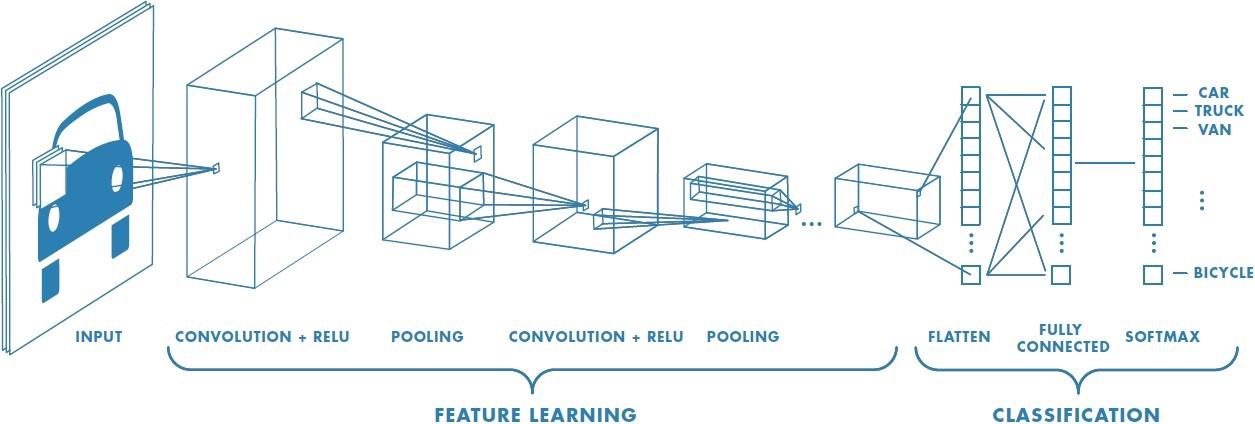
\includegraphics[width=150mm, keepaspectratio]{figures/cnn.jpeg}
    \caption{Egy konvolúciós neurális hálózat \cite{nnpic}}
\end{figure}

\subsection{Konvolúciós réteg}
Ebben a rétegben kétdimenziós konvolúciót végzünk a feldolgozandó képen. Ennek során először választunk egy kernelt. A kernel négyzetes mátrix, a képnél általában jóval kisebb mérettel. Gyakori kernelméret például a 3x3-as, vagy 5x5-ös mátrix. Alapvetően a kernel végighalad minden képkockán, és a középső pixelnek ad egy új értéket a kernel és a pixelek értékei alapján.

\begin{figure}[!ht]
    \centering
    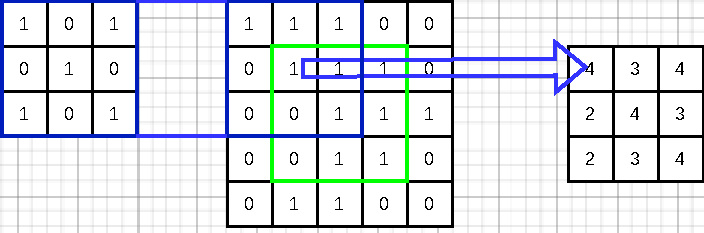
\includegraphics[width=150mm, keepaspectratio]{drawings/conv.drawio.pdf}
    \caption{2D konvolúció}
\end{figure}

Vegyük például a következő 3x3-as kernelt és egy kép 5x5-ös részletét. Az ábrán bal oldalt található a kernel, középen a bemeneti kép, jobb oldalon pedig a kimeneti kép. A képnek a zölddel jelölt részét tudjuk csak leképezni anélkül, hogy a kernel kimutatna a képen kívülre. Ezen a területen a kernel közepét a egy számmal helyettesítjük. Ezt a számot úgy képezzük, hogy a kernel értékeit megszorozzuk az fedésben lévő pixellel, majd ezeket az értékeket összeadjuk. Az új képen a kernel közepét ezzel az értékkel helyettesítjük. Ezután eggyel jobbra toljuk a kernelt, a sorvéget elérve pedig a következő sor elejére helyezzük.

Sok esetben szeretnénk csökkenteni a képek méretér a konvolúció során, hogy gyorsítsuk a hálózatot. Ehhez a konvolúció stride paraméterét kell növelnünk. A stride alapesetben 1, és azt jelzi, hogy a művelet elvégzése után mennyivel toljuk arrébb a kernelt. Könnyen belátható, hogy minél nagyobb a stride, annál kevesebb lesz a kimeneti pixelek száma, így csökken a kép mérete.

Jellemzően több konvolúció történik egymás után. Az első ilyen réteg feladata az alacsony szintű elemek megtalálása, például élek vagy színváltások megkeresése. Ahogy egyre több konvolúció történik egymás után, a hálózat egyre magasabb szintű jellegzetességeket fog tudni felismerni. Így már ebben a fázisban is az emberi megértéshez hasonlóan dolgozza fel a képeket a neurális hálózat.
\cite{ConvNetExplain}

\subsection{Pooling réteg}
A pooling rétegek feladata a bemenetük méretbeli csökkentése. Nagyon hasonlóan működnek a konvolúciós rétegekhez, a pooling rétegekben is egy kernel iterál végig a képen. Jellemzően egynél nagyobb stride értékkel.

A különbség a kernel értékeiben mutatkozik leginkább. Kétféle pooling-ot fordul elő gyakran. Átlag pooling esetében a kernelt az általa fedett pixelek átlagával helyettesítjük, maximum pooling esetében pedig a fedett pixelek közül a legnagyobbal. A maximum pooling a leggyakrabban használt a kettő variáció közül.

A pooling lényege tulajdonképpen a képen található domináns sajátosságok kinyerése. Ezekről a részekről forgatásra és pozícióra nézve invariáns információt tárol el a hálózat.\cite{ConvNetExplain}

\subsection{Teljesen összekötött réteg}
A teljesen összekötött réteg bármilyen neurális hálózat alapvető építőeleme. Ha a művelet kimenete nem egy másik kép, hanem valamilyen szöveges információ, például a képen látható objektum klasszifikációja, akkor a teljesen összekötött réteg végzi el az osztályba sorolás műveletét.

\begin{figure}[!ht]
    \centering
    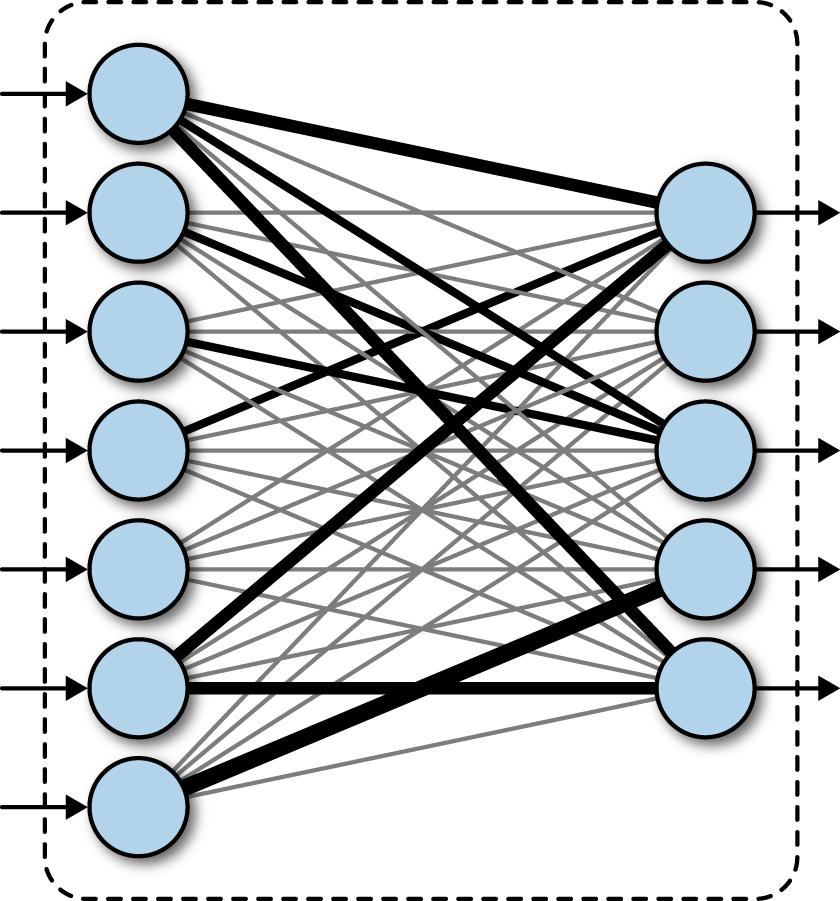
\includegraphics[width=80mm, keepaspectratio]{figures/fcl.png}
    \caption{Egy teljesen összekötött réteg \cite{ConvPic} }
\end{figure}

Ebben a rétegben két csoportba rendezve láthatunk neuronokat. A csoportok minden tagja össze van kötve a másik csoport összes tagjával és az összeköttetéseken súlyokat találunk. A képen a súlyokkal a vonalak vastagsága arányos. A jobb oldali csoport összes neuronja összegzi a bele futó élek végén található neuronok kimeneteit az éleken található értékekkel súlyozva, és az összeg lesz ennek a neuronnak a kimenete.

Ilyen rétegből is jellemzően több helyezkedik el egymás után. A legutolsó réteg a kimeneti réteg. Osztályozás esetén annyi kimeneti neuron van, ahány lehetséges osztály közül kell választani. Amelyik kimeneti neuronnak a legnagyobb az értéke, az ahhoz tartozó osztályba fogja sorolni a hálózat a bemeneti képet.

Felmerülhet kérdésként, hogy hogyan jutunk el egy képtől neuronokig. A kép a konvolúciós és pooling rétegekben folyamatosan egyre kisebb lesz méreteit tekintve. Egy ponton már olyan kicsi, hogy minden egyes pixelét tekinthetjük egy neuronnak, és felfoghatjuk a legelső teljesen összekötött réteg bemeneteként. A teljesen összekötött rétegek is jellemzően egymás után egyre kevesebb neuront tartalmaznak.

\section{Előre tanított neurális hálózat modellek}

A neurális hálózatok felhasználásának két lépése van. Először mintaadatok segítségével tanítani kell a hálózatot, ezután lehet csak kiértékelésre használni. A jelenlegi feladatnak csak a kiértékelés része az érdekes, ezt tudjuk ugyanis hatékonyan elvégezni a célhardveren.

Tanítás nélkül is van lehetőségünk neurális hálózatok felhasználására. Ebben az esetben ugyan nem tudjuk meghatározni, hogy milyen feladatot végez el a hálózat, azonban sok gyakori felhasználásra már rendelkezésre áll erősen optimalizált és teljesen tanított hálózat. Ezeket az előre tanított hálózatokat sok esetben van lehetőségünk áttanítani valamilyen másik, hasonló célra, azonban ebben a feladatban ilyen áttanítás nem lesz szükséges.

A Xilinx eszközök már sok esetben alkalmasak neurális hálózatok kiértékelésére. A cég mindenki számára elérhetővé tesz bizonyos neurális hálózat modelleket, amik olyan formátumban vannak, amiket Xilinx eszközön módosítás nélkül fel lehet használni kiértékelésre.
\cite{ModelZoo}

\subsection{Resnet50}
A modell teljes neve: \mycode{cf\_resnet50\_imagenet\_224\_224\_7.7G\_2.0}. A név a következő információkat tartalmazza: A modell caffe keretrendszerben volt tanítva az imagenet adathalmazon, resnet50 architektúrájú, és 224x224 pixel méretű képeken tud dolgozni. Ez a hálózat a bemenetére adott képet osztályozni tudja 10 lehetséges csoport közül egybe.

A feladatom első részében ezt a modellt használtam a rendszer tesztelésére, a pontos folyamatot a későbbiekben fogom bemutatni.

\subsection{Facerec}
A feladat további részeiben arcfelismerést és bounding box rajzolást kell majd elvégezni. A Model Zoo-t végignézve több lehetőség is adódik, ezek közül részletesebb tesztelés után fogok konkrét modellt választani. Mindegyikre igaz azonban, hogy a facerec arcfelismerő architektúrát valósítják meg. A különbség a bemeneti kép méretében, a tanító keretrendszerben és a tanításra felhasznált adathalmazban van.



\chapter{Xilinx ZCU106}
A feladat megoldására a Xilinx ZCU106 tesztkártyát használtam.\cite{ZCU106}

\begin{figure}[!ht]
    \centering
    \includegraphics[width=150mm, keepaspectratio]{figures/ZCU106.jpg}
    \caption{ZCU106 Tesztkártya}
\end{figure}

\section{Zynq UltraScale+ MPSoC}
A kártya központi egysége egy SoC (System on a Chip). Az SoC két részre osztható.

\begin{figure}[!ht]
    \centering
    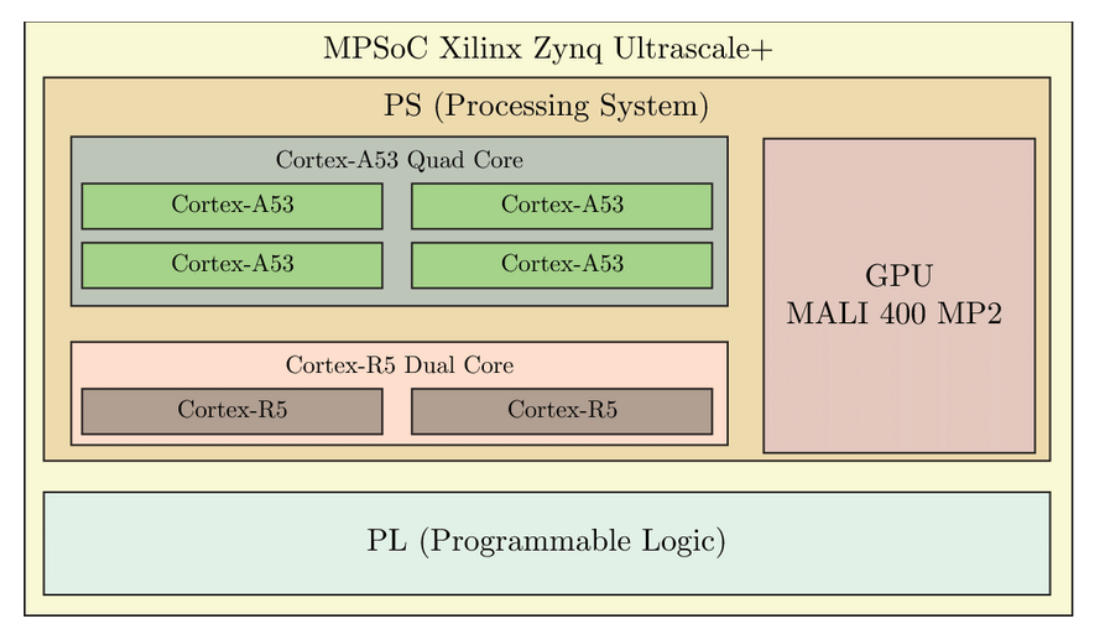
\includegraphics[width=150mm, keepaspectratio]{figures/PS.png}
    \caption{A Processing System blokkvázlata}
\end{figure}

A PL (Programmable Logic) részben, egy FPGA-hoz hasonlóan szabadon lehet hardvert kialakítani valamilyen hardverleíró nyelv segítségével. Ugyanakkor gyakori felhasználása a PL-nak, hogy nem írjuk meg kézzel a hardvert, hanem rendelkezésre álló IP (Intellectual Property) core-okat használunk fel. Az ilyen core-ok általában szoftverrel összhangban, az aktuális program valamilyen lépését képesek hardveresen gyorsítani. Elképzelhető még valamilyen interface, például HDMI interface kialakítása is. Ebben a feladatban leginkább a hardveres gyorsítás van a középpontban.

A PS (Processing System) részben általában leginkább CPU (Central Processing Unit) core-okat találunk. Ebben az SoC-ben található egy négymagos Arm Cortex-A53 processzor, és egy kétmagos Arm Cortex-R5 processzor. Előbbi az általános alkalmazások futtatására alkalmas, míg utóbbi képes valós idejű működésre is. A PS-t lehet használni bare metal alkalmazások futtatására, ebben az esetben a lefordított bináris alkalmazást közvetlenül a CPU-n futtatjuk. Lehetőség van azonban operációs rendszert futtatni a PS-en. Ebben a feladatban is ilyen megoldást választottam. Az operációs rendszer neve Petalinux, és egy későbbi fejezetben kerül majd bemutatásra.

A PS része még egy Arm MALI 400 MP2-es GPU is. A GPU feladata nem a hardveres gyorsítás, erre a célra a PL-ot kell felhasználni. A GPU segítségével lehetőség van videók dekódolására és enkódolására, valamint minimális grafikus megjelenítésre is.

\section{Perifériák és interface-ek}
A ZCU106 kártya számos perifériát tartalmaz, hogy az SoC-t a lehető legtöbb felhasználás esetében lehessen kipróbálni vagy tesztelni. Ezek közül a feladat szempontjából legfontosabbak fogom bemutatni.

\subsection{Memóriák}
A kártya rendelkezik két egységnyi DDR4 RAM memóriával is. Az egyik egy standard SoDIMM memória, amit a PS tud használni csakúgy mint egy normális számítógép. A másik egységen a memória chipek már nem rendelkeznek egy hordozó PCB-vel, hanem közvetlenül a kártyán helyezkednek el. Ezeket a memóriákat a PL-ból tudjuk elérni megfelelő hardver szintetizálásával.

\subsection{Nagysebességű interface-ek}
A kártyán jelen van szinte minden gyakran használt nagysebességű interface. Például rendelkezik egy 4 sávos 4. generációs PCIe csatlakozóval, RJ45 Ethernet csatlakozóval, valamint videó jeleknél használatos portokkal: egy HDMI és egy DisplayPort In/Out csatlakozóval.

A felsoroltak közül a feladat során fel lehet majd használni a DisplayPort csatlakozót, ezen keresztül is tudunk majd videó jelet küldeni az SoC-nak. Ezen kívül használni kell az Ethernet csatlakozót is, mivel a tesztelés során a kártyát távolról kell konfigurálni és az elérés Etherneten keresztül lehetséges.

\subsection{USB csatlakozók}
A kártyán található egy standard USB csatlakozó. A végső megoldás során valószínűleg a DisplayPort-os kamera helyett inkább egy USB interface-szel rendelkező kamera kerül majd felhasználásra.

A kártyán található egy micro-USB csatlakozó amit UART kapcsolat megvalósítására lehet felhasználni. A feladat során ennek is elkerülhetetlen a használata, hiszen ezen keresztül érjük majd el PS-en futó operációs rendszer CLI-ét (Command Line Interface).

\section{IP core-ok}
Az IP core-ok kicsit kilógnak a sorból, hiszen nincsenek rajta fizikailag a kártyán, viszont valamilyen módon mégis kapcsolódnak hozzá. Az IP core-okat a Xilinx szolgáltatja a tesztkártyákhoz, és ezek használata sokszor függ attól, hogy milyen módon vagy célra vásároltunk, és hogy milyen tesztkártyát.

A feladatban két lényeges IP core-t kell felhasználni. Az egyik a DPU (Deep Processing Unit), amit már az eddig elkészült tesztek során is fel tudtam használni. Ennek feladata, ahogy az a nevéből is látszódik, a mély neurális hálózatok, pontosabban ezek kiértékelésének hardveres gyorsítása.

A másik IP core felhasználása a tárgy második felében fog megvalósulni, ez a Multiscaler IP core lesz. Ennek feladata képek átméretezése.



% Acknowledgements
%~~~~~~~~~~~~~~~~~~~~~~~~~~~~~~~~~~~~~~~~~~~~~~~~~~~~~~~~~~~~~~~~~~~~~~~~~~~~~~~~~~~~~~
%\include{content/acknowledgement}


% List of Figures, Tables
%~~~~~~~~~~~~~~~~~~~~~~~~~~~~~~~~~~~~~~~~~~~~~~~~~~~~~~~~~~~~~~~~~~~~~~~~~~~~~~~~~~~~~~
%\listoffigures\addcontentsline{toc}{chapter}{\listfigurename}
%\listoftables\addcontentsline{toc}{chapter}{\listtablename}


% Bibliography
%~~~~~~~~~~~~~~~~~~~~~~~~~~~~~~~~~~~~~~~~~~~~~~~~~~~~~~~~~~~~~~~~~~~~~~~~~~~~~~~~~~~~~~
\addcontentsline{toc}{chapter}{\bibname}
\bibliography{bib/mybib}


% Appendix
%~~~~~~~~~~~~~~~~~~~~~~~~~~~~~~~~~~~~~~~~~~~~~~~~~~~~~~~~~~~~~~~~~~~~~~~~~~~~~~~~~~~~~~
\include{content/appendices}

%\label{page:last}
\end{document}
